% ----------------------------------------------------------
% Referencial Teórico
% ----------------------------------------------------------
\chapter{Referencial Teórico}

\section{Planejamento Racional de Fármacos}
Devido aos avanços da biologia, atualmente o processo de descoberta e desenvolvimento de novos compostos químicos capazes de prevenir ou curar doenças passou a seguir um planejamento racional, com embasamento lógico e teórico \cite{rdd}. Esse processo é denominado “Planejamento Racional de Fármacos” (do inglês RDD - \emph{Rational Drug Design}) e, de acordo com Kuntz \cite{kun92}, ele se divide em quatro etapas e está reprensentados através do \emph{workflow} da Figura \ref{fig:rddworkflow} \cite{kar11}: 

\begin{figure}[h]
	\center
	\includegraphics[width=14cm]{images/rdd_workflow.png}
	\caption{\emph{Workflow} do processo de planejamento racional de fármacos assistido por computador \cite{kar11}}
	\label{fig:rddworkflow}
\end{figure}


\begin{enumerate}
  \item O primeiro passo é definir um receptor (normalmente uma proteína) \cite{dre00} e analisar computacionalmente sua estrutura 3D. A estrutura da proteína é determinada por cristalografia por difração de raios X ou ressonância magnética nuclear \cite{far99}, sendo as informações resultantes armazenadas em um banco de dados como o Protein Data Bank - PDB \cite{ber00}. Essa análise tem por objetivo localizar possíveis regiões de ligação onde um ligante pode estabelecer ligações (atividades 1 e 2 do \emph{workflow} da Figura \ref{fig:rddworkflow});
  
  \item Baseado nas prováveis regiões de ligação identificadas no passo anterior, é selecionado um conjunto de possíveis candidatos, chamados ligantes (usualmente pequenas moléculas que podem ser buscadas em Banco de Dados de compostos como o ZINC \cite{irw05}) que podem se ligar a essa região no receptor (atividade 3 \emph{workflow} da Figura \ref{fig:rddworkflow}). As diferentes conformações que determinado ligante pode assumir dentro do sítio de ligação de uma determinada proteína são simuladas por softwares de docking como AutoDock 3.05 \cite{mor98} (atividade 4 do \emph{workflow} da Figura \ref{fig:rddworkflow});
  
  \item Os ligantes que teoricamente obtiveram melhores resultados nas simulções são experimentalmente sintetizados e testados (atividade 5 do \emph{workflow} da Figura \ref{fig:rddworkflow});
  
  \item Baseado nos resultados experimentais, o medicamento é gerado (atividade 6 do \emph{workflow} da Figura \ref{fig:rddworkflow}) ou o processo retorna ao passo 1.
  
\end{enumerate}
  
  Estas quatro etapas descritas por Kuntz \cite{kun92} contemplam apenas as fases de pesquisa e desenvolvimento de um novo medicamento. 
Somente após um longo período de pesquisas e testes \emph{in-vitro} e \emph{in-vivo}, estabelecendo eficácia e segurança, o novo fármaco é submetido para registro no órgão regulador.

A Tabela \ref{tab:rddtempo} apresenta, de uma forma geral, as etapas que envolvem o processo de desenvolvimento de um novo fármaco e o tempo médio de cada uma delas \cite{kun92}.

% Please add the following required packages to your document preamble:
% \usepackage{booktabs}
\begin{table}[h]
	\caption{Passos e tempo para desenvolvimento de um novo fármaco \cite{kun92}}
	\label{tab:rddtempo}
	\centering
	\begin{tabular}{@{}lc@{}}
	\toprule
	\multicolumn{1}{c}{\textbf{Passo}}      & \textbf{Tempo (Anos)} \\ \midrule
	Descoberta e geração de um candidato    & 1 - 2                 \\
	Otimização do candidato                 & 1 - 2                 \\
	Ensaios in-vitro e in-vivo              & 1 - 2                 \\
	Testes toxicológicos                    & 1 - 3                 \\
	Testes de segurança em humanos          & 1                     \\
	Testes de eficiência em humanos         & 1 - 2                 \\ \midrule
	\textbf{Tempo total de desenvolvimento} & \textbf{6 - 12}       \\ \bottomrule
	\end{tabular}
\end{table}

O desenvolvimento de fármacos auxiliado por computador (do inglês CADD - \emph{Computer-aided drug design}) consiste na utilização de recursos, ferramentas e técnicas computacionais contribui de forma significativa para as etapas de desenvolvimento de um fármaco.  Diferentes estágios deste processo podem ser beneficiados pelo uso da computação, podendo ser aplicado na identificação da molécula-alvo, planejamento, análise e melhoramento de ligantes.


\section{Dinâmica Molecular}

O advento da utilização de recursos computacionais aplicado às áreas medicinais e biológicas têm proporcionado o avanço de técnicas e uso de ferramentas que contribuem de forma expressiva para o planejamento racional de fármacos.

A Dinâmica Molecular (DM) é uma técnica de simulação computacional, fundamentada nos princípios da Mecânica Clássica, que possibilita o estudo do comportamento dinâmico microscópico de um sistema molecular, em diferentes intervalos de tempo \cite{nam08}. 

A simulação por DM fornece informações dos átomos que constituem o sistema molecular, permitindo o cálculo de diversas propriedades (pressão, temperatura, volume, energia livre, etc) e análise do potencial de interação dos ligantes na estrutura e estabilidade das proteínas \cite{kar11}.

De acordo com Lesk \cite{art08}, as interações entre os átomos em uma molécula podem ser classificadas de duas maneiras:

\begin{quote}
	(a) Ligações químicas primárias - interações fortes entre átomos que estão localizados bem próximos no espaço. São consideradas interações fixas pois são consistentes em um grande número de conformações, não sendo desfeitas ou alteradas quando a conformação de uma proteína muda. 

	(b) Interações mais fracas que dependem da conformação, podem ser significativas em algumas conformações e não em outras - elas afetam conjuntos de átomos que são aproximados devido a diferentes padrões de enovelamento da cadeia.
\end{quote}

As proteínas são corpos flexíveis que não possuem uma conformação única e fixa. Elas apresentam conformações que variam em um intervalo de tempo. A Figura \ref{fig:dm} ilustra a flexibilidade da enzima receptora InhA, onde cada cor representa uma conformação em um determinado instante de tempo \cite{COH10}.

\begin{figure}[h]
	\center
	\includegraphics[scale=0.4]{images/dm_inha.png}
	\caption{Flexibilidade da enzima receptora InhA. Sobreposição de diferentes conformações da InhA, representadas em fitas, durante uma simulação de DM. A conformação inicial da simulação está representada pela cor verde. Outras duas conformações foram capturadas pela simulação de DM nos intervalos de 1,000 ps (cor azul) e 3,000 ps (cor magenta). O retângulo tracejado identifica a região com maior flexibilidade \cite{REN13}.}
	\label{fig:dm}
\end{figure}

A conformação de uma proteína pode ser especificada pela lista de átomos na estrutura, por suas coordenadas e pelo conjunto de ligações químicas entre eles. A avaliação de uma conformação é feita através do cálculo de conjuntos de potenciais de energia. Estes calculos são computacionalmente complexos e intensivos, mas com a evolução rápida da capacidade de processamento dos computadores esta técnica é beneficiada diretamente \cite{art08}.

A simulação por DM se mostra um método versátil e acessível, sendo considerada a melhor técnica para geração de um conjunto de conformações de um receptor \cite{kar11}. Devido à isso, os dados dos conjuntos de conformações dos receptores utilizados neste trabalho foram gerados utilizando a DM.


\section{Docagem Molecular}

A Docagem Molecular é considerada um dos principais processo do CADD, e é através dela que são produzidos os dados detalhados sobre a interação entre receptores e seus ligantes \cite{LEN96}. 

No processo de Docagem Molecular, algoritmos de docagem são executados para testar e analisar virtualmente a interação entre um ligante e um receptor. Estes algoritmos geram um grande número de interações, onde em todas elas, o ligante é testado em diferentes orientações e conformações dentro do sítio de ligação do receptor, de modo a formar um complexo estável. 
Usualmente o receptor é uma proteína ou uma molécula de ácido nucléico, e o ligante pode ser uma pequena molécula ou até mesmo outra proteína. A Figura \ref{fig:docking} \cite{ALE13} ilustra cada um destes elementos e apresenta como é feita a interação entre eles.

\begin{figure}[h]
	\center
	\includegraphics[width=17cm]{images/docking.png}
	\caption{Representação do processo de docagem molecular em três dimensões (3D) entre uma proteína como receptor e uma pequena molécula como ligante, na qual se estabelece uma interação entre eles no sítio de ligação do receptor \cite{ALE13}.}
	\label{fig:docking}
\end{figure}

Diversas interações devem ser testadas para que seja identificado o melhor encaixe do ligante no sítio de ligação do receptor, ou então, a região ou o sítio de ligação deve ser previamente conhecido. Um dos critérios utilizados para avaliar as interações é pelo cálculo da energia livre de ligação (do inglês FEB - \emph{Free Energy of Binding}). Quanto mais negativo for o valor resultante, melhor é a ligação estabelecida \cite{kar07}. A Figura \ref{fig:tcldock} \cite{REN13} ilustra o processo de docagem em três dimensões, a posição inicial da molécula do ligante TCL no sítio de ligação da molécula InhA e a posição do ligante TCL após a simulação de docagem molecular.

\begin{figure}[h]
	\center
	\includegraphics[scale=0.60]{images/TCLdocking.png}
	\caption{Representação da superfície molecular do sítio de ligação da enzima receptora InhA na estrutura de cristal. O ligante TCL é  representado na forma de palitos. A conformação inicial do ligante TCL aparece em cor laranja, e a conformação final após uma simulação de docagem molecular é representada em ciano \cite{REN13}.}
	\label{fig:tcldock}
\end{figure}

As primeiras abordagens envolvendo a docagem entre proteínas e ligantes consideravam ambos elementos como sendo corpos rígidos. O modelo conhecido como "chave e fechadura" (do inglês \emph{lock-and-key}, proposto por Emil Fisher em 1894, prevê um encaixe perfeito do ligante no sítio de ligação do receptor, tal como uma chave encaixa em sua fechadura correspondente \cite{kar07}. 

No entanto, ambos proteína e ligante são moléculas flexíveis. Desta forma, o modelo histórico de "chave e fechadura" deu seu lugar à novas teorias, as quais passaram a considerar totalmente ou parcialmente a flexibilidade do ligante e do receptor \cite{SOU06}. Atualmente um dos maiores desafios na área de docagem molecular é conseguir manipular, de forma eficience, a flexibilidade do receptor da proteína. A eficiência da busca pela melhor conformação é determinada pelo número de graus de liberdade  \cite{SOU06}. 

Considerar a flexibilidade do ligante não requer um grande esforço computacional, pois geralmente são moléculas pequenas que possuem poucos átomos em sua estrutura \cite{COH10}. No entanto, a consideração da flexibilidade de ambos receptor e ligante se torna um complicador para os cálculos da docagem molecular, se tornando um problema computacional devido a complexidade e ao tamanho da proteína receptora \cite{art08}.

Existem diversos estudos e abordagens que contemplam a flexibilidade do receptor em simulações de docagem molecular. Entretanto, no presente trabalho, os dados utilizados foram previamente desenvolvidos no LABIO (Laboratório de Bioinformática, Modelagem e Simulação de Biossistemas) combinando técnicas de docagem molecular com dados resultantes de simulações por DM. A partir disso, foi gerado um conjunto de \emph{snapshots} sequenciais que representam as diferentes conformações da proteína receptora InhA em um intervalo de tempo.bilidade do ligante \cite{kar11}.

\section{Modelagem OLAP}

Com o desenvolvimento tecnológico, ficou cada vez mais fácil a obtenção de dados sobre um determinado assunto. Atualmente, qualquer aparelho eletrônico é capaz de gerar uma imensa massa de dados. Porém, estes dados se tornam irrelevantes se não estiverem devidamente organizados e não possuirem uma ferramenta capaz de tratá-los. Para as organizações, o tratamento destes dados significa transformá-los em algo que possa agregar valor.

Um sistema de suporte à decisão (do inglês OLAP - \emph{On-line Analytical Processing}) é uma ferramenta que permite analisar os dados \emph{on-line} de forma multidimensional, auxiliando a tomada de decisão nos mais diversos níveis, sejam eles operacionais, táticos e estratégicos. De acordo com com Turban \emph{et al.} \cite{TUR05}, o OLAP se define em “uma categoria ampla de aplicações e técnicas para coletar, armazenar, analisar, fornecer acesso aos dados e ajudar os usuários da empresa a fazerem melhores negócios e tomarem melhores decisões estratégicas”. 

A representação dos dados em um modelo OLAP é como uma matriz. Cada dimensão é caracterizada por uma questão de negócio e sempre considera-se uma dimensão para o tempo. Também é possível que uma dimensão possua hierarquia, por exemplo, a dimensão tempo pode ter: ano, semestre, mês, dia, etc. Nestas dimensões os dados são agregados, mas é possível navegar entre as hierarquias de modo que os dados sejam exibidos com um maior nível de granularidade. A ação de ir de um nível genérico para um mais detalhado é chamado de \emph{drill-down}. A ação inversa é chamada de \emph{drill-up}.

Um modelo dimensional implementado em um banco de dados relacional é representado fisicamente por tabelas, e caracteriza-se pelo modelo do tipo estrela (do inglês \emph{Star Schema}) devido à forma que a sua estrutura está organizada. Este tipo de modelo possui como principal característica o relacionamento entre diversas tabelas de dimensão e uma tabela de fatos centralizada \cite{KIM13}.

Quando o modelo dimensional passa a ser implementado em um banco de dados multidimensional, sua representação é na forma de um cubo. Um cubo OLAP pode ser equivalente ou derivado de um modelo do tipo estrela \cite{KIM13}. A Figura \ref{fig:starVSolap} ilustra a organização estrutural dos dados utilizando o modelo estrela e o modelo em cubo.

\begin{figure}[h]
	\center
	\includegraphics[width=14cm]{images/starvsolap.png}
	\caption{Representação da organização estrutural dos dados nos modelos do tipo estrela e cubo. (Material adaptado de \cite{KIM13})}
	\label{fig:starVSolap}
\end{figure}

As dimensões representam os elementos "quem, o quê, onde, quando, como e porquê" de um processo de negócio de uma organização, por exemplo: "produto", "vendedor" e "loja". Cada dimensão possui uma chave primária e um conjunto de atributos que descrevem de forma textual os elementos envolvidos no processo de negócio. Os atributos servem para detalhar as características de uma dimensão e são essenciais para auxiliar na tomada de decisão \cite{KIM13}. Utilizando como exemplo a dimensão "produto", ela poderia conter os atributos "nome", "preço" e "categoria".

A tabela fato é onde as informações produzidas pela execução de um processo de negócio são armazenadas. Estas informações são chamadas de métricas ou medidas. As métricas geralmente são valores numéricos, pois os dados são agregados utilizando operações de somatório, média, etc. Cada entrada em uma tabela fato, corresponde a uma entrada em cada uma das dimensões \cite{KIM13}. A Figura \ref{fig:exOlap} ilusta um modelo relacional do tipo estrela.

\begin{figure}[h]
	\center
	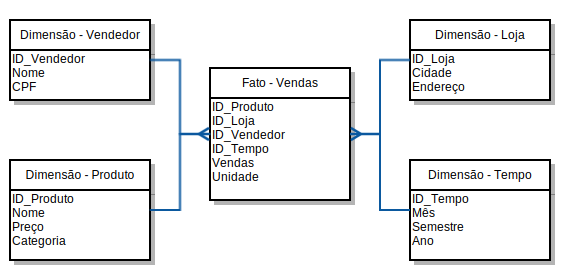
\includegraphics[width=13cm]{images/ex_olap.png}
	\caption{Representação de um modelo dimensional em um banco de dados relacional do tipo estrela.}
	\label{fig:exOlap}
\end{figure}

Os dados armazenados em um cubo OLAP passam por algoritmos de indexação, técnicas de armazenamento e outras otimizações que fazem com que as consultas realizadas nesta estrutura de dados, mesmo sendo complexas, tenham um alto desempenho no tempo de resposta para o usuário.

Um dos processo que fazem parte da modelagem de dados OLAP é o de extração, transformação e carga (do inglês ETL - \emph{Extract, Transform and Load}). Este processo consiste na extração de dados de fontes externas e na transformação dos mesmos, para que possam atender às necessidades de negócio. Posteriormente, estes dados são carregados em um \emph{Data Warehouse} ou em outros ambientes de banco de dados.

O processo de ETL é considerado o mais complexo e que consome mais tempo durante a criação de um ambiente de \emph{Data Warehouse/Business Intelligence}, pois consiste em movimentar e transformar os dados que irão servir como base para futuras decisões gerenciais. Portanto, os dados precisam estar precisos e consistentes. 
Muitas vezes as informações estão armazenadas em diferentes fontes de dados e não possuem um padrão de estrutural de dados \cite{KIM13}. Nestes casos, as etapas de extração e transformação precisam de um esforço para que os dados sejam tratados de forma homogênea.























